\documentclass[a4paper,10pt,twoside]{cpc-hepnp}

\usepackage{multicol}
\usepackage{graphicx}
\usepackage{booktabs}
\usepackage{amssymb,bm,mathrsfs,bbm,amscd}
\usepackage[tbtags]{amsmath}
\usepackage{lastpage}
\usepackage{lineno}
\usepackage{ifpdf}
\usepackage{subfigure}
\ifpdf
   \DeclareGraphicsRule{*}{mps}{*}{}
\else
   \DeclareGraphicsRule{*}{eps}{*}{}
\fi

\linenumbers

\renewcommand{\mathstrut}{\protect\vphantom{\hat{0123456789}}}

\linespread{2} % comment this after all the revision 
\begin{document}



\fancyhead[c]{\small Chinese Physics C~~~Vol. xx, No. x (201x) xxxxxx}
\fancyfoot[C]{\small 010201-\thepage}

%\footnotetext[0]{Received 14 March 2009}


\title{Fast simulation of the CEPC conceptual detector with  {\textsc{Delphes}} and its validation 
\thanks{The study was partially supported by the CAS/SAFEA International Partnership Program for Creative Research Teams¬and funding from CAS and IHEP for the Thousand Talent and Hundred Talent programs, as well as grants from the State Key Laboratory of Nuclear Electronics and Particle Detectors.}}

\author{%
      Xin. Mo$^{1)}$%
\quad Gang. Li$^{1;2)}$\email{li.gang@ihep.ac.cn}%
\quad Manqi. Ruan$^{1;3)}$\email{manqi.ruan@ihep.ac.cn}%
\quad Xinchou. Lou$^{1,2)}$%
}
\maketitle


\address{%
$^1$ Institute of High Energy Physics, Chinese Academy of Sciences, Beijing 100049, China\\
$^2$ University of Texas at Dallas, Richardson, TX 75080-3021, USA
}


\begin{abstract}
In this paper, the {\textsc{Delphes}~} is used to simulate the detector on the Circular Electron-Positron Collider (CEPC). The geometry and performance of the CEPC detector are presented. The fast simulation in the {\textsc{Delphes}~} framework is validated with  a few benchmark processes, including $\mu\mu H$ and $H$ to inclusive decay,  $q\bar{q}H$ and $H$ to invisible, and $\nu\bar{nu}$ and $H$ decaying via double W bosons. The comparisons between {\textsc{Delphes}~} and the full simulation, which is based on Geant4 \& Marlin, shows that the Dephes can simulate CEPC detector well.  
\end{abstract}


\begin{keyword}
CEPC, {\textsc{Delphes}~}, Fast simulation
\end{keyword}

\begin{pacs}
%1---3 PACS(Physics and Astronomy Classification Scheme, http://www.aip.org/pacs/pacs.html/)
13.66.Fg, 14.80.Bn, 07.05.-t
\end{pacs}

\footnotetext[0]{\hspace*{-3mm}\raisebox{0.3ex}{$\scriptstyle\copyright$}2013
Chinese Physical Society and the Institute of High Energy Physics
of the Chinese Academy of Sciences and the Institute
of Modern Physics of the Chinese Academy of Sciences and IOP Publishing Ltd}%

%\begin{multicols}{2}



\section{Introduction}\label{sec:intro}
CEPC\cite{ref:cepc_det, ref:cepc_acc} is a next generation electron-positron collider proposed by Chinese scientists.
The machine is expected to collide electron and positron beams at the center-of-mass energy of 240- 250 GeV to maximize the Higgs production cross section through the $e^+e^− \to ZH$ process, with an instantaneous luminosity of $2\times10^{34}$ cm$^{-2} s^{-1}$.
CEPC is designed to deliver a total of 5 ab$^{-1}$ integrated luminosity to two detectors in 10 years, over $10^6$ Higgs events will be produced during this period. 
The large statistics with clean backgrounds will enable CEPC to perform Higgs precision measurements, 
Standard Model (SM) tests, and searches for potential new physical phenomenons.
 In order to investigate  sensitivity to new physics, theorists would get involved and various new models would be tested. To save computing time and to simplify  the procedure of full detector simulation and reconstruction,  a dedicated fast simulation tool is highly demanded. 

{\textsc{Delphes}~}\cite{ref:delphes} is a fast simulation framework  developed in 2009, and the latest prime version was released in 2013, which is designed for phenomenological studies on the simulation of various detector designs.  The {\textsc{Delphes}~} framework simulates the response of a detector composed of an inner tracker, electromagnetic and hadron calorimeters, and a muon system. All are organized concentrically with a cylindrical symmetry around the beam axis. The energy and momentum are smeared according to the resolutions of detector. Eventually, all kinds of particles are reconstructed with algorithm based on PFA\cite{ref:pfa} philosophy, then clustering into jets with FastJet~\cite{ref:fastjet} .

This paper is organized as following.  In Sect.{~\ref{sec:detector}}, the CEPC detector concept are introduced briefly.  Then in Sect.{~\ref{sec:simulation}}, the MC generation, full simulation of detector,  and framework reconstruction are summarized. In Sect.{~\ref{sec:validation}}, some benchmark processes are chosen to the validate the simulation of  the {\textsc{Delphes}~} on CEPC by comparing the fast and full simulaitons, including  $e^+e^- \to \mu^+\mu^- H$  and Higgs $\to $inclusive, $e^+e^- \to q\bar{q} H$ with Higgs decaying into invisible, $e^+e^- \to \nu\bar{\nu} H$ with Higgs coupling to W boson pair, and $e^+e^\to ZH \to 2(q\bar{q})$. In the end the conclusion remarks are presented. 

\section{CEPC detector conceptual design\label{sec:detector}}

The CEPC detector concept design\cite{ref:cepc_det}  takes the ILC detector, ILD\cite{ref:ilc, ref:ild},  as a reference and adopts the philosophy of PFA, which benefits from a high granularity  calorimetric system. 

The CEPC detector consists of three main sub-detectors and a superconducting solenoid of 3.5 T.  The three sub-detectors are, from inner to outer,  a hybrid tracking system composed of several silicon based devices and a Time Projection Chamber (TPC), a high granularity calorimetry system, and a Muon detector. 

The hybrid tracking system has five parts.  A vertex detector (VTX), constructed with high spatial pixel sensor, is placed very close to the interaction point (IP) and  the inner radius is only 16 mm. The VTX provides very precision measurements of the IP position of tracks and events, which is used for the $b-/c-$jet flavor tagging and $\tau$-tagging.  A Silicon Inner Tracker (SIT) is just outside  and cooperating with the VTX for vertex reconstruction and flavor tagging. A set of Forward Tracking Disks (FTDs)  are placed in the forward region to increase the geometric acceptance of tracking system with coverage up to $|\cos\theta| = 0.99$.  A Silicon External Tracker (SET) and End-cap Tracking Disks (ETD) are taken as the outermost layer of whole tracker system, which provide precision position measurements of tracks entering the calorimetric system.  The TPC, with a 2.35m half-length and 1.8m outer radius, provides about 200 hits per track and 100$\mu$m resolution in $r\phi$ plane, which allow for excellent pattern recognition,  track reconstruction efficiency, and potential $dE/dx$-based particle identification. 

A calorimetric system consisting of Electromagnetic Calorimeter (ECAL) and Hadron Calorimeter (HCAL) with very fine granularity is placed inside the solenoid. The system plays an essential role in the Particle-Flow Algorithm (PFA), providing excellent separation of showers from different particles and jet energy resolution of 3-4\%. 

A superconducting solenoid of 3.5 T is surrounding the calorimetry system. The return yoke is placed outside the solenoid. The CEPC muon system acts as the muon identifier, the solenoid flux return yoke and the support structure for the whole spectrometer. High muon detection efficiency, low hadron mis-identification rate, modest position resolution and large coverage are the main concerns of the design.

%\begin{enumerate}
%\item A vertex detector(VTX), constructed with high spatial resolution pixel sensor, the inner radius is 16mm, used for flavor-tagging and $\tau$-tagging.
%\item A silicon tracker system, which contains:
%\begin{enumerate}
%\item[-] Silicon Inner Tracker(SIT), corperating with VTX for vertex reconstruction and flavor-tagging.
%\item[-] Forward Tracking Disks(FTDs), increasing the geometric acceptance of the tracking system with coverage of $|\cos\theta|<0.99$.(But the coverage of calorimeters is merely $|\cos\theta|<0.985$, which is used in fast simulation).
%\item[-] Silicon External Tracker(SET) and End-cap Tracking Disks(ETDs), providing more arm length of the tracker system, thus improving the track momentum resolution of charged particles.
%\end{enumerate}
%\item A Time Projection Chamber(TPC), with a 2.35m half-length and 1.8m outer radius. It could provide about 200 hits per track and 100$\mu$m resolution in $r\phi$ plane.
%\item A calorimetry system, which consists of Electromagnetic Calorimeter(ECAL) and Hadron Calorimeter(HCAL). It is an essential role in the Particle-Flow Algorithm(PFA), is designed to excellent separation of showers and reach of $3\%\sim4\%$ resolution for jet energy.
%\item A Muon system is surrounding outside of the calorimetry system.
%\end{enumerate}


\section{Monte Carlo generation, detector simulation and reconstruction \label{sec:simulation}}

For CEPC detector design and optimization, a whole set of $ZH$ signal processes and Standard Model (SM) backgrounds have been prepared\cite{ref:cepccpc} with generic Monte-Carlo generator {\sf Whizard 1.95}{~\cite{ref:whizard}}.  To simulate the detector response, a full simulation package, Mokka{~\cite{ref:mokka}}, based on Geant4{~\cite{ref:geant4}} and a fast simulation framework with {\textsc{Delphes}~}{~\cite{ref:delphes}} are used.  The Particle Flow Algorithm (PFA) philosophy is utilized in the reconstruction of both the full and fast simulation.

%In order to validate the configuration of Delphes for the CEPC, some benchmark processes are chosen for the comparison. The first one is the Higgs inclusive decay process in the associated Z leptonic channel, which is critical for Higgs model independent measurement. The second one is the Higgs invisible decay mode, associated with hadronic Z decay channel. This channel may be sensitive to some new physics related to Higgs. The last one is Higgs decays into double W bosons, one is on-shell meanwhile the other is off-shell, and the associated Z decays into neutrinos. This benchmark channel can be valuable to constrain the SM parameters, such as HWW coupling.

After full simulation,  hits in different sub-detector are digitized properly and reconstructed with reconstruction software framework Marlin{~\cite{ref:marlin}}.   A dedicated PFA, Arbor\cite{ref:arbor},  is adopted for particle reconstruction, and the alternative PFA, Pandora{~\cite{ref:pandora}}, is taken as reference. Jets are reconstructed with LCFIPlus package\cite{ref:lcfiplus}, where a $e^+e^-~k_t$ algorithm{~\cite{ref:eekt}},  often referred to also as {\sf Durham} algorithm,  is used for jet-clustering. 

The detector model implemented in the {\textsc{Delphes}} is same as the one in full simulation but with some necessary simplifications. For the charged tracks simulated with {\textsc{Delphes}}, there is a common strategy to smear their momentum. The angular resolution is assumed to be perfect, so that the smearing only applied to the transversal momentum. In practice, the resolution of their momentum is described as a Gaussian, which is parameterized function of $p_t$ and $\eta$. The values for the simulation is $\sigma=\sqrt{0.001^2+(10^{-5}p_t)^2}$ as required in CEPC pre-CDR. Then the charged tracks are  reconstructed according to the user-defined probability, which are listed in Tab.~\ref{tab:tab1}.
\begin{center}
\tabcaption{\label{tab:tab1}Efficiencies for charged tracks(\%)}
\begin{tabular}{@{}*{3}{ll}}
\hline \hline
		& $P_t\le0.1$ & $P_t>0.1$ \\ \hline\hline
$\eta\le3.0$  & 0 		     & 100  \\
$\eta>3.0$    & 0 		     & 0 \\
\hline \hline
\end{tabular}
\end{center}




For neutral objects which mainly rely on the calorimetric system, some points should be emphasized: 1. The fake rate for electrons, muons and photons is not implemented in the current version of {\textsc{Delphes}~}; 2. The photon conversions into electron-positron pairs are ignored neither. Both the true photons and electrons reaching calorimeter without a reconstructed track are considered as photon in {\textsc{Delphes}~}.

The overall reconstruction of particles implemented in {\textsc{Delphes}~} is mainly based on a perfect PFA . For the charged tracks, the reconstruction involves both the tracker system and the calorimetric system. Since the resolution of tracking system is better than this of calorimeter in the CEPC energy region, it can be convenient to use the tracking information within the tracker acceptance for estimating the charged particles momenta. The efficiencies could be parameterized as a function of the energy and pseudo-rapidity. For a preliminary study, the present parameters are listed in Tab.~\ref{tab:tab2}, which are consistent those of full simulation and reconstruction.
\begin{center}
\tabcaption{\label{tab:tab2}Effciencies for identification of $\gamma$, $e^{\pm}$, $\mu^{\pm}$}
\begin{tabular}{@{}*{3}{ll}}
\hline \hline
		& Energy$\le2.0$ & Energy$>2.0$ \\ \hline\hline
$|\eta|\le1.5$  & 0 		     & 0.99 \\
$1.5<|\eta|\le3.0$    & 0 	     & 0.99 \\
$|\eta|>3.0$  & 0 		     & 0      \\
\hline \hline
\end{tabular}
\end{center}

\iffalse
\begin{center}
\tabcaption{\label{tab:arbor}Migration matrix from Arbor}
\begin{tabular}{@{}*{3}{ll}}
\hline \hline
\%	    & $e$ & $\mu$ & $\pi$ \\ \hline\hline
$e$      & 99.91$\pm$0.08  & 0.08$\pm$0.03   & $<10^{-5}$ \\
$\mu$  & $<10^{-5}$ 	      & 99.60$\pm$0.19 & 0.39$\pm$0.19 \\
$\pi$    & 0.34$\pm$0.17    & 0.25$\pm$0.14   & 99.39$\pm$0.22  \\
\hline \hline
\end{tabular}
\end{center}
\fi

In Delphes, two sets of 4-vector are provided with PFA, which are named as {\it{particle flow tracks}} and {\it{particle flow towers}}. For each particle flow object, $E_{ECAL}$, $E_{HCAL}$ and $E_{ECAL, trk}$, $E_{HCAL, trk}$ are essential for the particle flow reconstruction. $E_{ECAL}$, $E_{HCAL}$ are the total energy deposited in electromagnetic calorimeter and hadronic calorimeter, $E_{ECAL, trk}$, $E_{HCAL, trk}$ are also the total energy deposited in the calorimeters, but from the charged particle whose track has been reconstructed. Then a quantity $E^{eflow}_{tower}$ is defined as
\begin{eqnarray}
&\Delta_{ECAL}=E_{ECAL}-E_{ECAL, trk}, \quad\Delta_{HCAL}=E_{HCAL}-E_{HCAL, trk}\\
&E^{eflow}_{tower}=\mathrm{max}(0,\Delta_{ECAL})+\mathrm{max}(0,\Delta_{HCAL})
\end{eqnarray}
So for a neutron particle like photon, the particle flow tower can be simply created with the energy $E_{ECAL}$ or $E_{HCAL}$. Meanwhile, for a charged particle,  if $E_{E,HCAL}\le E_{E,HCAL,trk}$, only a particle flow track will be reconstructed with the energy $E_{E,HCAL,trk}$; if $E_{E,HCAL}>E_{E,HCAL,trk}$, a particle flow track with $E_{E,HCAL,trk}$ and a particle flow tower with $E^{eflow}_{tower}$ will be reconstructed simultaneously.

In order to get same performance of jet-clustering, $e^+e^-~k_t$ algorithm is also used for the results of fast simulation. The exclusive mode of fast jet is used and  all input particles are forced into fixed number of jets without any $y_{ij}$ or $P_t$ cuts, which can be applied at analysis stage.  

\section{Validation with full simulation\label{sec:validation}}

\iffalse
On the CEPC, the full simulation is achieved with Geant4 and several toolkits based on the LCIO framework\cite{ref:lcio}. Geant4\cite{ref:geant4} is a general simulation package suitable from single particle phenomena study to full scale detector simulation. In the current study, the geometric structure and material information of the CEPC have been encoded as CEPC\_v1 configuration card, which is essentially for simulating the detector responds with Geant4. After the digitization, the detector responds are stored in the form of LCIO format. A user interface of LCIO, named as Marlin, is provided to read all the data from simulation and reconstruct them as hits, tracks, and clusters.

Tracks and clusters then will be interpreted as the reconstructed particles with Arbor algorithm\cite{ref:arbor}. The basic idea of Arbor algorithm is inspired by the fact that the shower spatial development  in the calorimeter follows the topology of a tree. In calorimeter, if the distance of a pair of hits is less than a predefined threshold, a connector will be established for the pair. To avoid loop connectors or multiple connectors to a single hit, a cleaning procedure is implemented to ensure that at each hit there is at most one connector which with minimum angle to a well selected direction. After all tree structure of shower completed, the shower would be merged with a track if it is charged or not.
\fi

The simulation and reconstruction in {\textsc{Delphes}~} has to be validated by comparing the resolution of output objects to those of full simulation, as well as the efficiencies. Three  benchmark processes are selected for the validation, which cover all the main physics objects of CEPC experiments, such as tracks, photons, and (multi-)jets final sates.   

For this purpose, all the relevant distributions should be compared to check the shapes, the resolutions, and efficiencies.    In these plots, the outputs from {\textsc{Delphes}~} approximately agree with the full simulation cases, some points should be mentioned:

\subsection{$e^+e^-\to \mu^+\mu^-h$} For $\mu^+\mu^-h$ channel and $q\bar{q}h$ channel, the di-muons and di-jets come from Z boson decay, and Higgs is tagged from the recoiling side, so the invariant mass of those systems represent Z meanwhile the recoiling mass is Higgs. But in $nnh\to WW^*$, the Z boson decays invisibly into neutrinos, all the visible information comes from $WW^*$ and eventually from Higgs, so in Fig.~\ref{fig:nninva} and Fig.~\ref{fig:nnreco} the invariant mass represent Higgs and recoiling side is Z.

\begin{center}
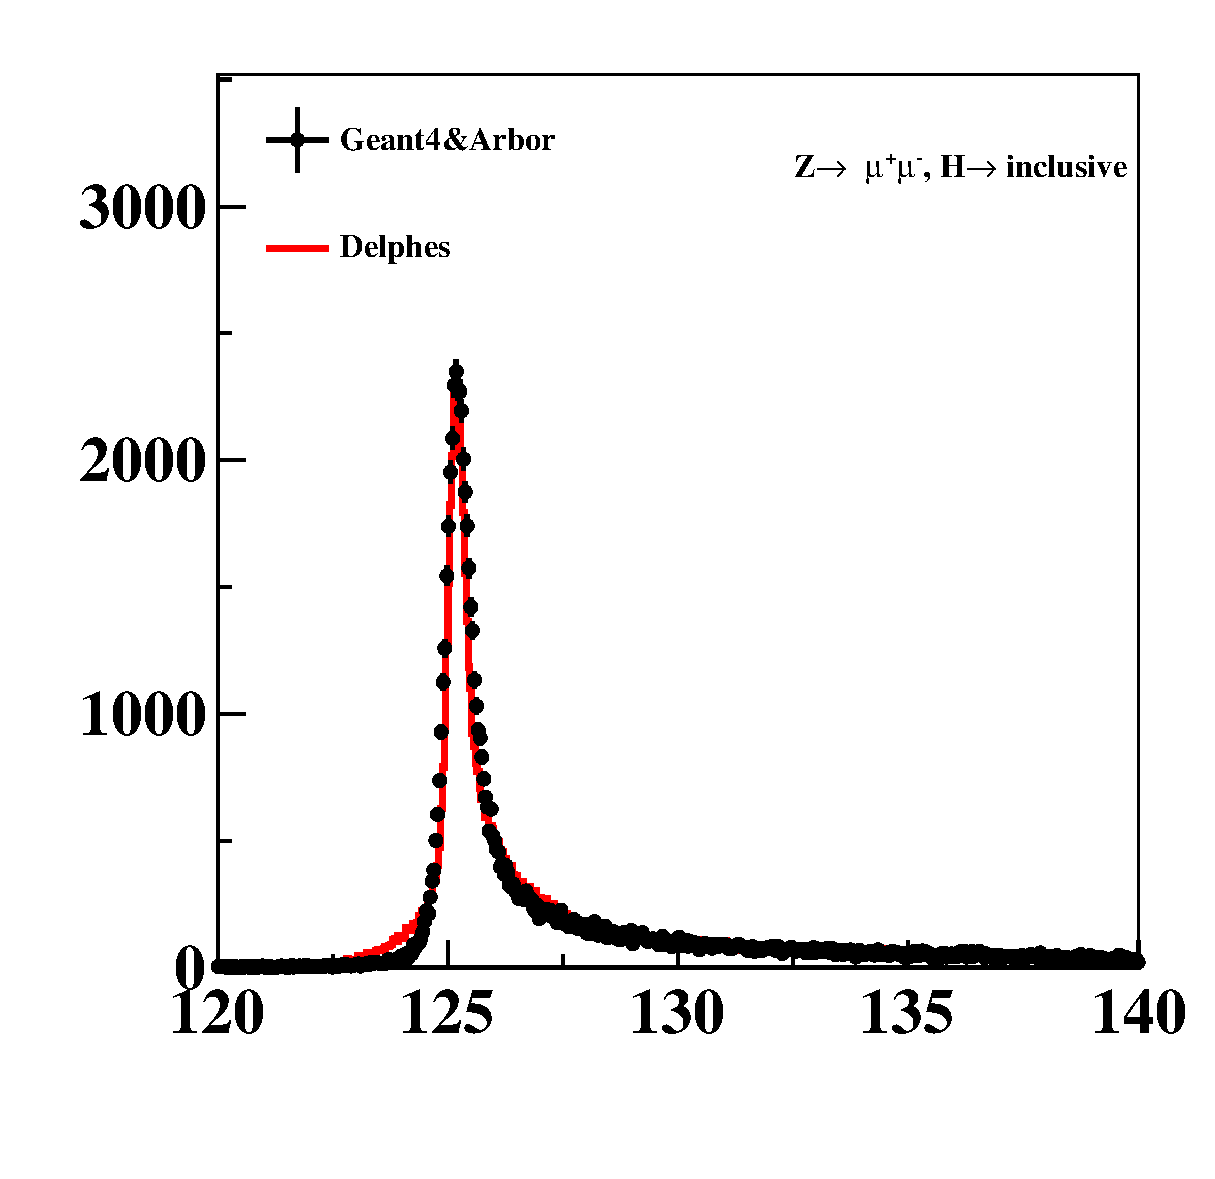
\includegraphics[width=0.9\linewidth]{e2e2h_reco}
\figcaption{\label{fig:mumureco} Recoiling mass against $\mu^+\mu^-$.}
\end{center}
\begin{center}
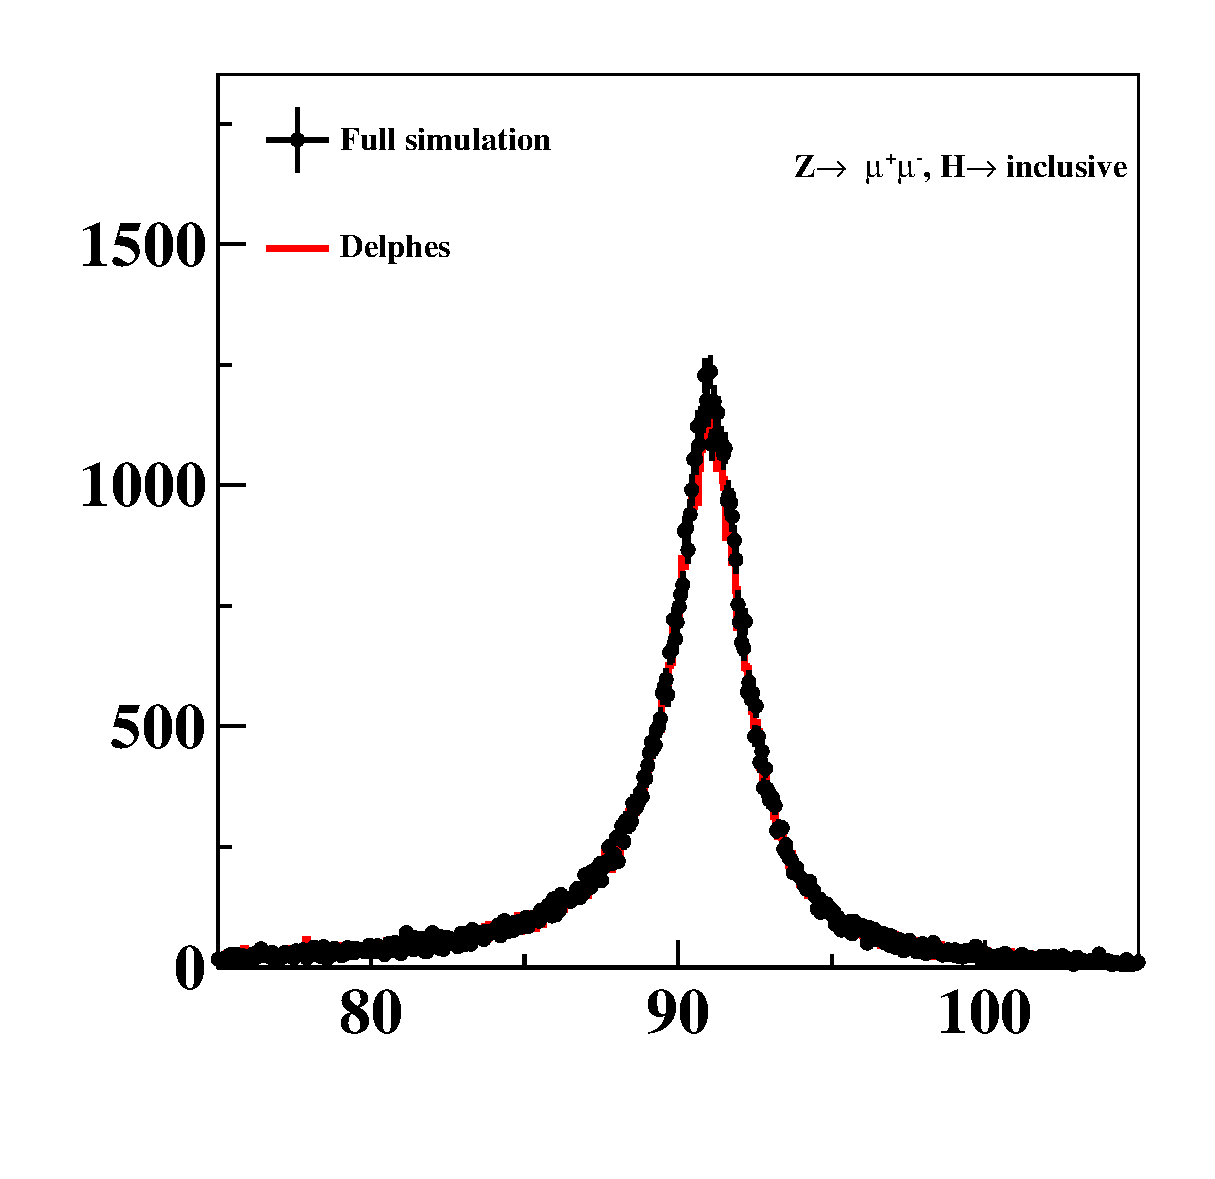
\includegraphics[width=0.9\linewidth]{e2e2h_mass}
\figcaption{\label{fig:mumuinva} Invariant mass of $\mu^+\mu^-$.}
\end{center}

\subsection{$e^+e^-\to q\bar{q}h, h \to\mbox{invisible}$ and $e^+e^-\to \nu\bar{\nu}H, H\to q\bar{q}$}
The Z mass in $q\bar{q}h$ channel is rescaled after Arbor's output, the final effect of the rescaling is a translation from right to left in X axis. This operation could be considered as an calibration for the reconstruction scheme. 


\begin{center}
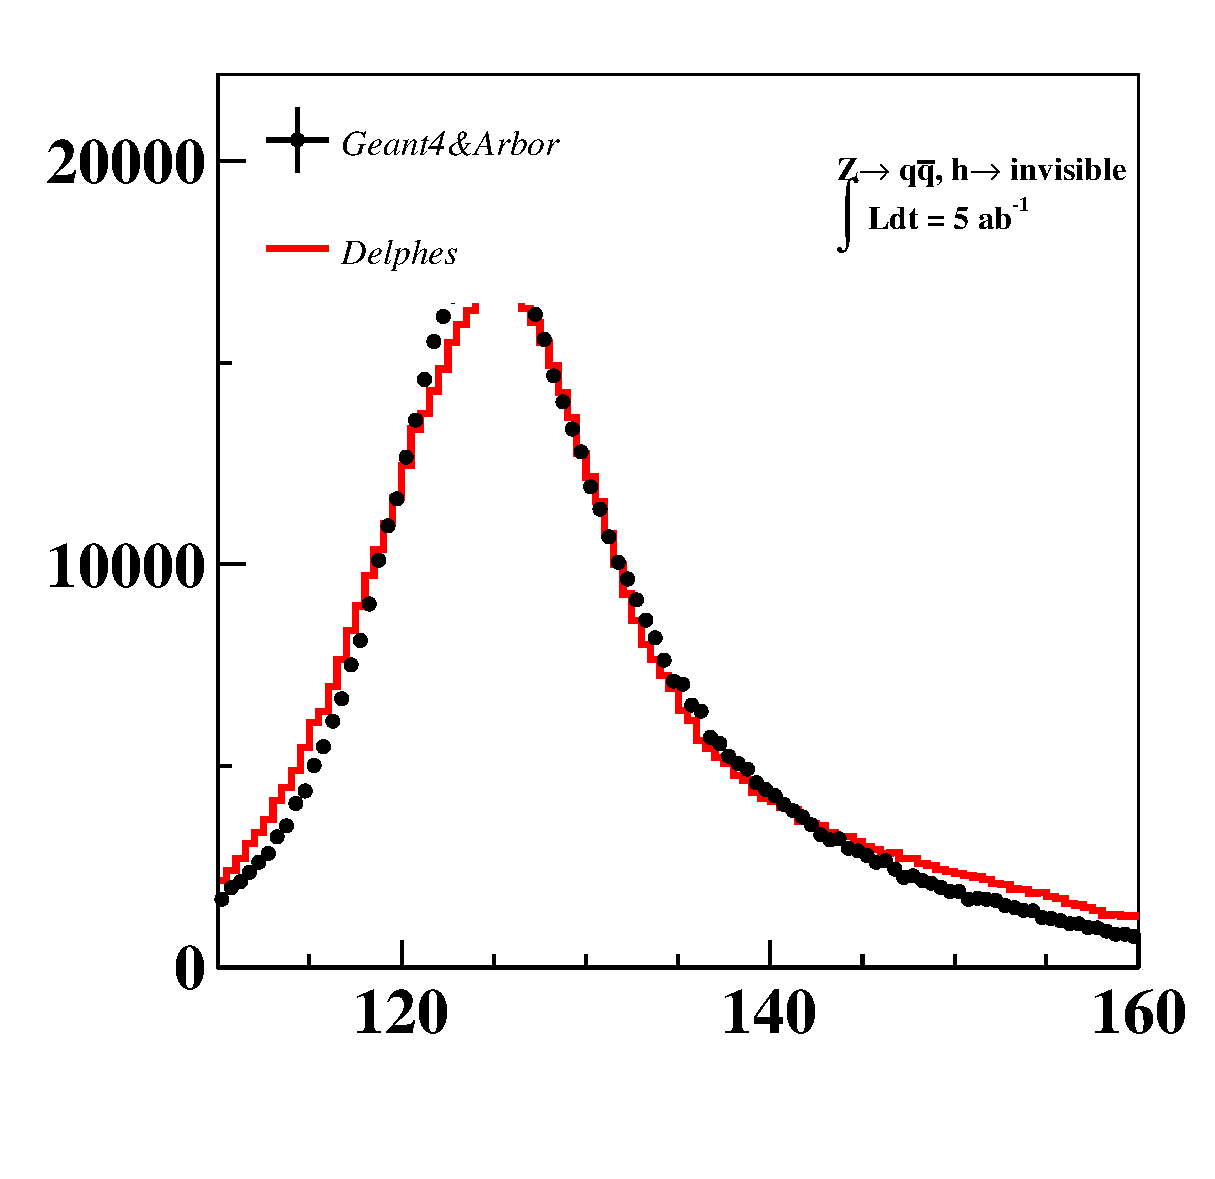
\includegraphics[width=0.9\linewidth]{qqh_reco}
\figcaption{\label{fig:qqreco} Recoiling mass against $q\bar{q}$.}
\end{center}
\begin{center}
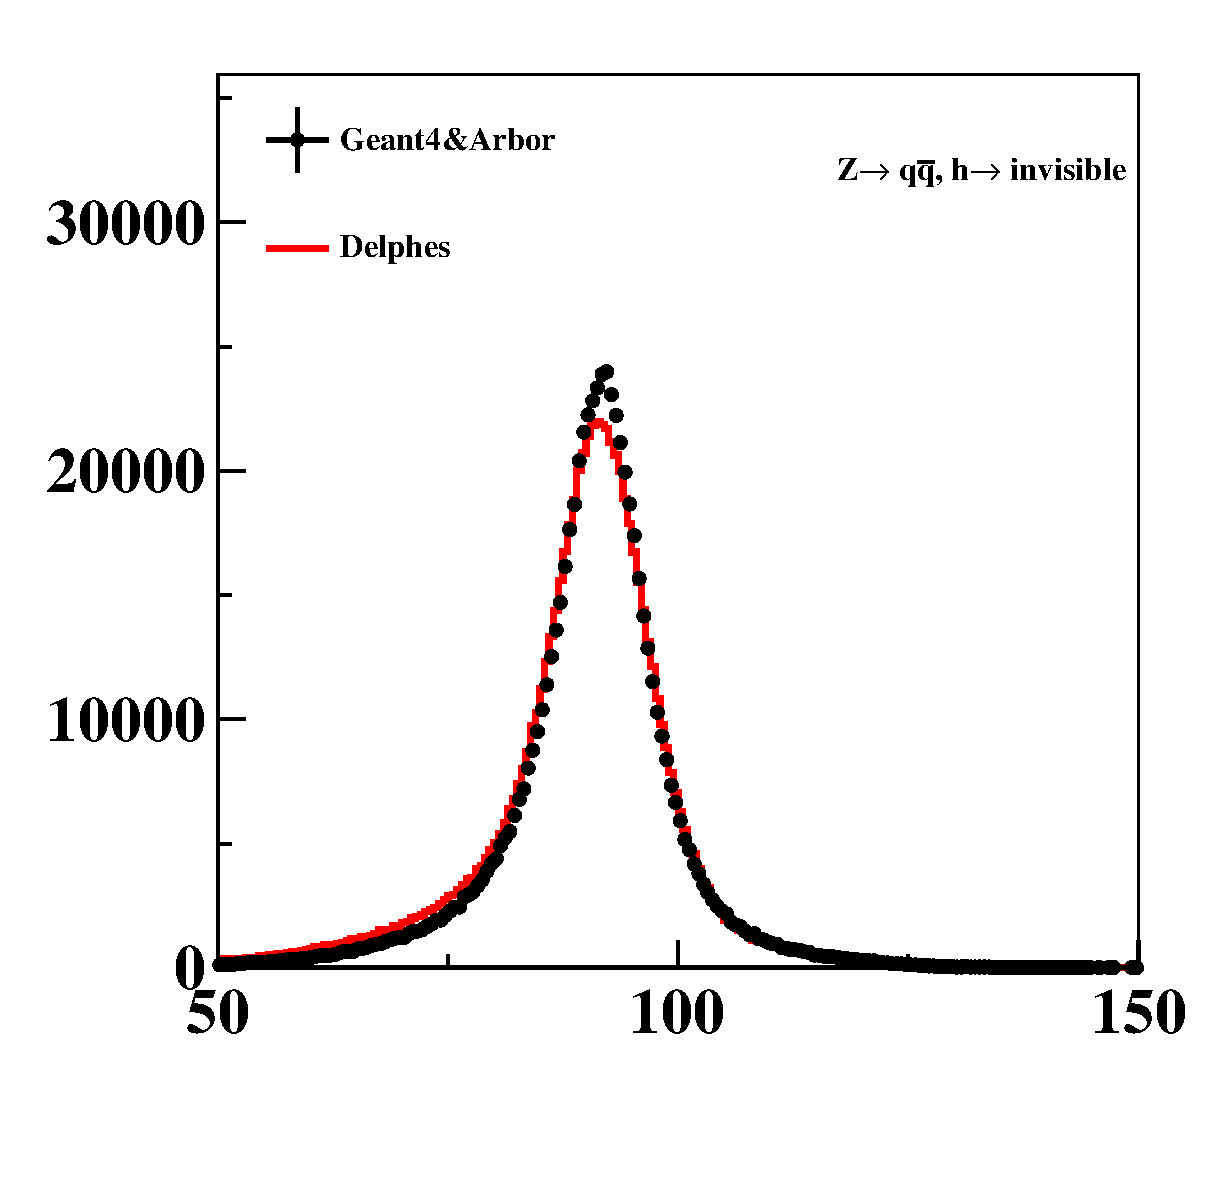
\includegraphics[width=0.9\linewidth]{qqh_mass}
\figcaption{\label{fig:qqinva} Invariant mass of $q\bar{q}$.}
\end{center}

\begin{center}
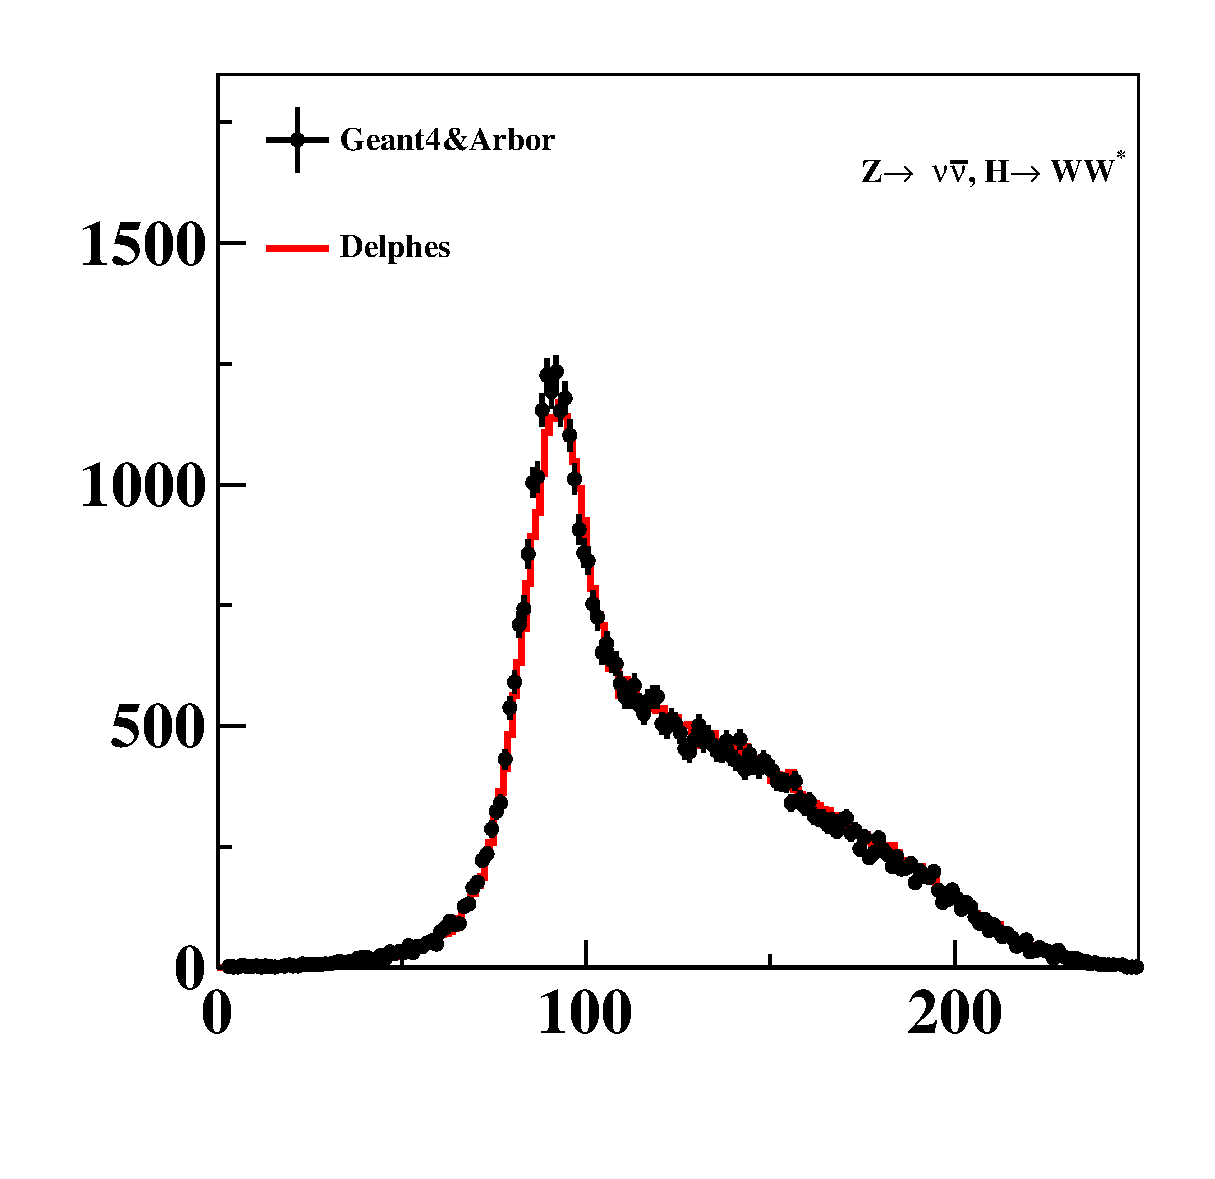
\includegraphics[width=0.9\linewidth]{nnh_reco}
\figcaption{\label{fig:nnreco} Recoiling mass against $WW^{*}$ in $n\bar{n}h\to WW^{*}$.}
\end{center}
\begin{center}
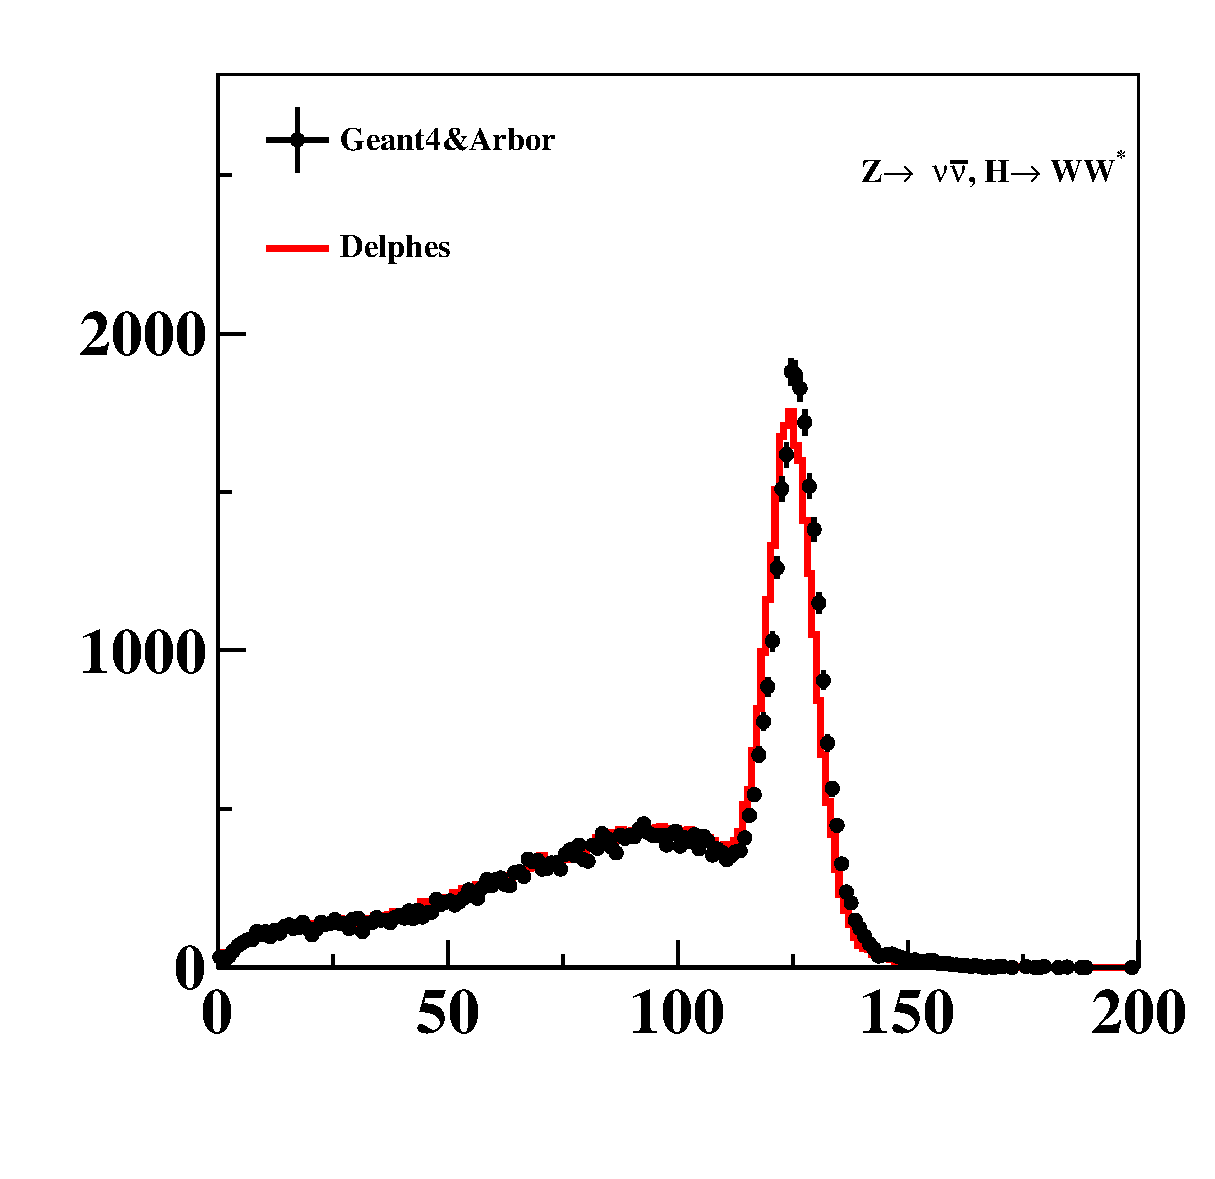
\includegraphics[width=0.9\linewidth]{nnh_mass}
\figcaption{\label{fig:nninva} Visible mass in $n\bar{n}h\to WW^{*}$.}
\end{center}

\subsection{$e^+e^-\to ZH\to 2(q\bar{q})$}

\begin{center}
\includegraphics[width=0.9\linewidth]{full_vs_delphes_z}
\figcaption{\label{fig:zjj} Invariant mas of jet pair, peaking at $Z$ mass.}
\end{center}
\begin{center}
\includegraphics[width=0.9\linewidth]{full_vs_delphes_h}
\figcaption{\label{fig:hjj} Invariant mas of jet pair, peaking at Higgs mass}
\end{center}


\begin{center}
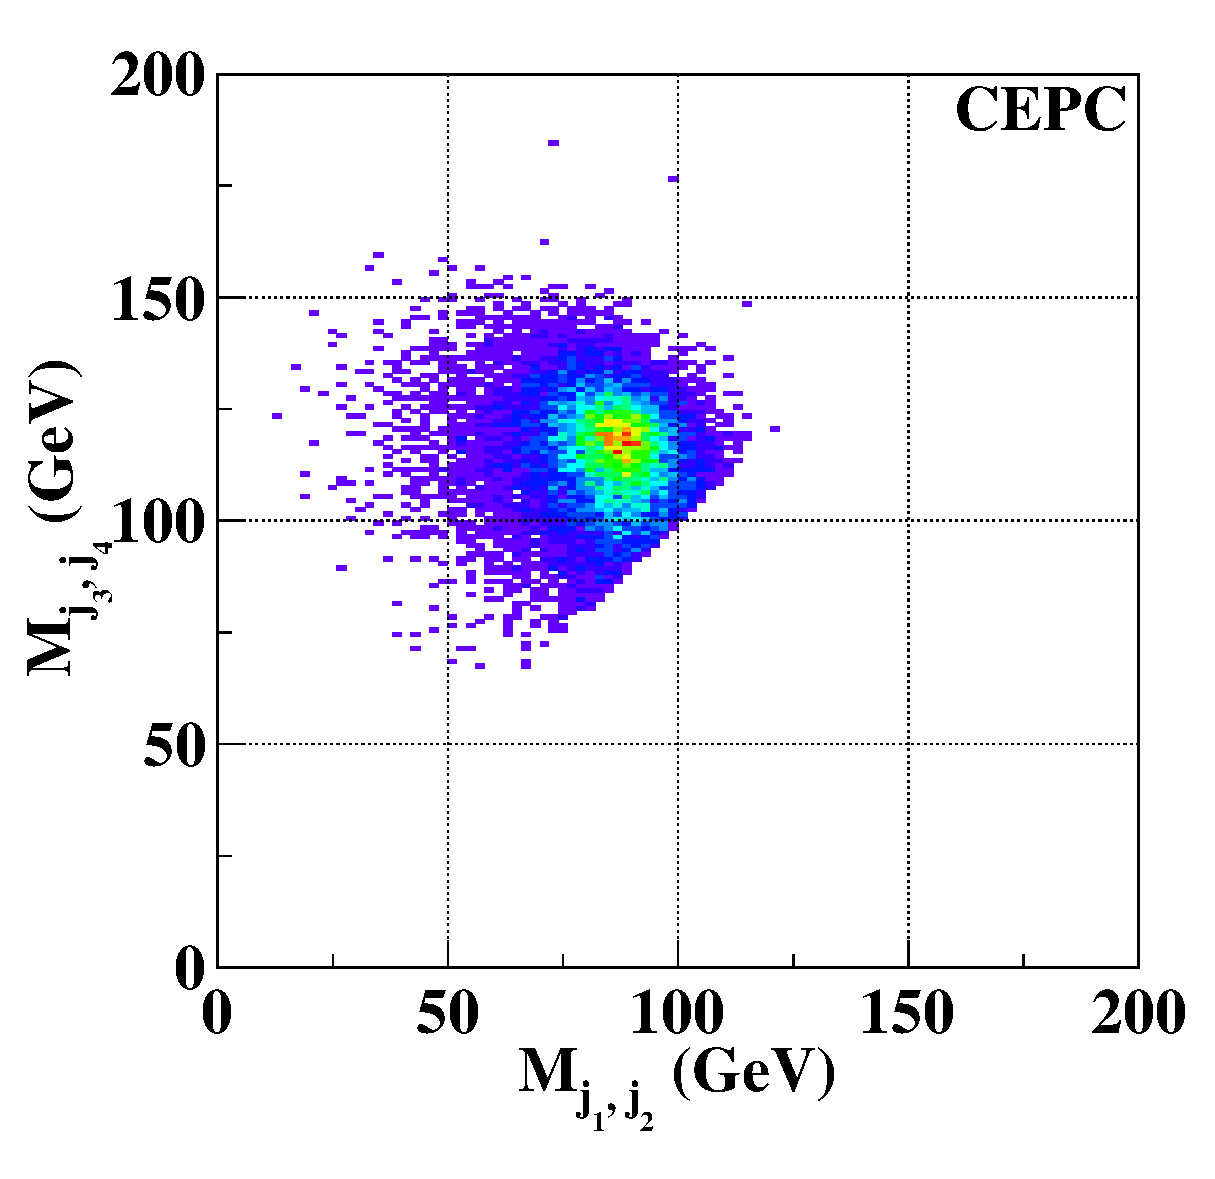
\includegraphics[width=0.9\linewidth]{Full2DCOL}
\figcaption{\label{fig:zjj} Scattering plot of $M_{j_1,j_2}$ vs. $M_{j_3,j_4}$ for full simulation}
\end{center}
\begin{center}
\includegraphics[width=0.9\linewidth]{Fast2DCOL}
\figcaption{\label{fig:hjj} Scattering plot of $M_{j_1,j_2}$ vs. $M_{j_3,j_4}$  for fast simulation }
\end{center}

\section{Conclusion\label{sec:conclusion}}
To validate the flexibility of {\textsc{Delphes}~} on CEPC, a comparison between {\textsc{Delphes}~} simulation and Geant4 \& Arbor has been studied in this paper. In the current study, the results agree very well with our previous understanding for full simulation of CEPC. It should be noted that the {\textsc{Delphes}~} parametrization has not been all covered in this study, such as those related to flavor tagging. Meanwhile, most of the parameters have to be determined with the feedback from the full simulation.
\vspace{3mm}

\begin{thebibliography}{90}

\vspace{3mm}

\bibitem{ref:cepc_det}CEPC-SppC Preliminary Conceptual Design Report: Physics and Detector, by the CEPC Study Group.
\bibitem{ref:cepc_acc}CEPC Accelerator Preliminary Conceptual Design Report, by the CEPC Study Group.
\bibitem{ref:delphes}S. Ovyn, X. Rouby,  V. Lemaitre, {\textsc{Delphes}~}, a framework for fast simulation of a generic collider experiment, arXiv:0903.2225 [hep-ph].
\bibitem{ref:pfa}P. Janot, Particle Flow Event Reconstruction from LEP to LHC, Presented at Excellence in Detectors and Instrumentation Technologies workshop, CERN, 2011.
\bibitem{ref:ilc}T. Abe et al., The International Large Detector: Letter of Intent, arXiv:1006.3396 [hep-ex].
\bibitem{ref:ild}T. Behnke et al., The International Linear Collider Technical Design Report - Volume4:Detectors,arXiv:1306.6329 [physics.ins-det].
\bibitem{ref:cepccpc}X. Mo, G. Li, M. Ruan, X. Lou, Physics cross sections and event generation of $e^+e^?$ annihilations at the CEPC, Chi. Phys. C, 2016, {\bf 40}: 033001.
\bibitem{ref:whizard}W. Kilian, T. Ohl, J. Reuter, Eur. Phys. J. C, 2011, {\bf 71}:1742.
\bibitem{ref:mokka}  P.~Mora de Freitas and H.~Videau, LC-TOOL-2003-010.
\bibitem{ref:geant4}S. Agostinelli et al., GEANT4: A simulation toolkit, Nucl. Instrum. Meth. A, 2003, {\bf 506}:250.
\bibitem{ref:marlin} http://ilcsoft.desy.de/portal/software\_packages/marlin/index\_eng.html
\bibitem{ref:arbor}M. Ruan, H. Videau, Arbor, a new approach of the Particle Flow Algorithm, arXiv:1403.4784 [physics.ins-det]
\bibitem{ref:pandora} 
  M.~A.~Thomson,
  Nucl.\ Instrum.\ Meth.\ A {\bf 611}, 25 (2009)
  doi:10.1016/j.nima.2009.09.009
  [arXiv:0907.3577 [physics.ins-det]].
\bibitem{ref:lcfiplus} 
  T.~Suehara and T.~Tanabe,
  Nucl.\ Instrum.\ Meth.\ A {\bf 808}, 109 (2016)
  doi:10.1016/j.nima.2015.11.054
  [arXiv:1506.08371 [physics.ins-det]].
\bibitem{ref:eekt} S. Catani, Y. L. Dokshitzer, M. Olsson, G. Turnock and B. R. Webber, Phys. Lett. B {\bf 269}, 432 (1991);
%\bibitem{ref:antikt}M. Cacciari, G. P. Salam, G. Soyez, JHEP,2008, {\bf 04} :063 [arXiv:0802.1189 [hep-ph]].
\bibitem{ref:fastjet}M. Cacciari, G. P. Salam, Phys. Lett. B, 2006, {\bf 641}:57 [hep-ph/0512210], M. Cacciari, G.P. Salam, G. Soyez, Eur. Phys. J. C, 2012, {\bf 72}:1896[arXiv:1111.6097].
\bibitem{ref:lcio}F. Gaede, T. Behnke, N. Graf, T. Johnson, arXiv:physics/0306114.

\end{thebibliography}
%\end{multicols}

\clearpage

\end{document}
